\section*{Introdução}

No âmbito da unidade curricular de Administração de Redes, implementamos a rede descrita na figura \ref{fig:rede}.

\begin{figure}[h]
\centering
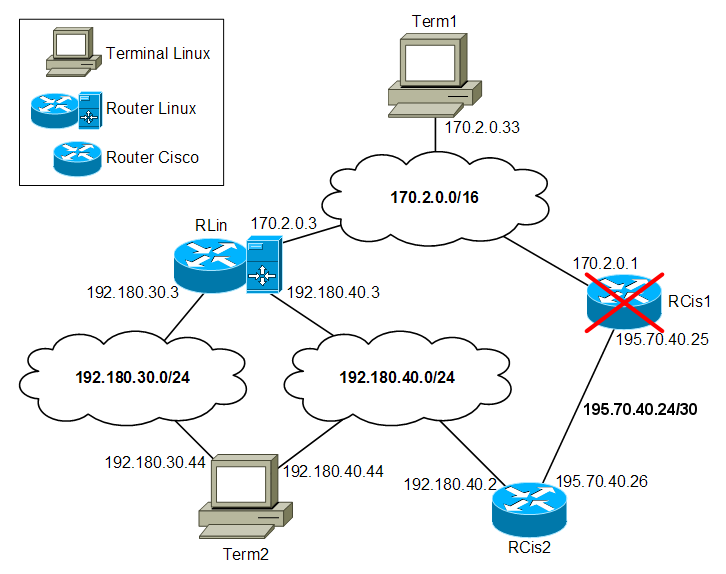
\includegraphics[width=0.7\textwidth]{rede.png}
\label{fig:rede}
\caption{Rede implementada na aula.}
\end{figure}

As máquinas \textsf{Term1}, \textsf{Term2} e \textsf{RLin} foram concretizadas com 3 \emph{workstations} Fedora 23, cada uma com as necessárias interfaces de rede. A máquina \textsf{RCis2} consiste num \emph{router} Cisco 1841.

A rede \textsf{170.2.0.0/16} consiste na ligação direta entre uma interface de \textsf{RLin} e \textsf{Term1}.
A rede \textsf{192.180.30.0/24} foi implementada com uma ligação direta entre \textsf{RLin} e \textsf{Term2}.
A rede \textsf{192.180.40.0/24} foi implementada com um \emph{switch} ligado a \textsf{RLin}, \textsf{Term2} e \textsf{RCis2}. 
